\documentclass[runningheads]{llncs}
\usepackage{amsmath,amssymb}
\usepackage{booktabs}
\usepackage{graphicx}
\usepackage{hyperref}

\begin{document}

\title{Selective Prediction and the Persistence Illusion:\\
A Diagnostic Decomposition of VIX Regime Classification}

\titlerunning{Selective Prediction and the Persistence Illusion}

\author{Anonymous}
\authorrunning{Anonymous}
\institute{Anonymous}

\maketitle

\begin{abstract}
Confidence-based selective prediction systems for financial regime
classification can achieve apparent accuracy exceeding 90\% while providing
no genuine predictive skill beyond naive persistence. We demonstrate this
through a systematic diagnostic study of VIX regime classification across
5{,}000 trading days (July 2006--May 2026). A six-component evaluation
protocol reveals that a three-feature HAR-style logistic regression matches
or exceeds a 36-feature Random Forest at four of five prediction horizons
under moving-block bootstrap testing. A coverage-matched persistence rule
makes identical predictions to the Random Forest on every jointly covered day
at horizons $N \geq 10$ (McNemar $b = c = 0$), confirming that accuracy
gaps reflect coverage composition rather than multi-feature predictive skill.
The confidence filter achieves 0\% accuracy on calm-to-high volatility
transitions at all horizons; explicit cost-weighting up to $20\times$ does
not improve this. SHAP attribution assigns 71.9\% of prediction mass to
VIX autocorrelation features, and a two-layer LSTM also fails on transition
days. Results replicate on S\&P~500 trend regimes, establishing the
persistence illusion as a structural property of selective prediction on
serially correlated labels. The diagnostic protocol is modular and applicable
to any selective prediction system on autocorrelated outcomes.
\keywords{Selective prediction \and Persistence illusion \and VIX regime
classification \and Random Forest \and Autocorrelation artifact \and
Volatility forecasting \and Explainable AI}
\end{abstract}


\section{Introduction}

The CBOE Volatility Index (VIX) measures the 30-day implied volatility of
S\&P~500 options and is widely used by risk managers and policymakers to
monitor equity market uncertainty~\cite{whaley2009}. A VIX reading below 20
is conventionally associated with calm market conditions, while readings
above 20 signal elevated fear and uncertainty. Classifying whether VIX will
exceed this threshold at some future horizon is a natural machine learning
task with direct applications to portfolio risk management, options hedging,
and dynamic asset allocation.

Confidence-based selective prediction---which allows classifiers to abstain
when prediction confidence is low~\cite{chow1970,geifman2017}---is a natural
fit for this setting. By reserving predictions for high-confidence days and
abstaining otherwise, selective systems can trade coverage for reliability.
Published studies regularly report accuracy figures of 85--95\% for
Random Forest or Gradient Boosting classifiers on VIX regime data,
seemingly validating the practical utility of such approaches.

This paper argues that these headline figures constitute a diagnostic
rather than an achievement. On autocorrelated binary time series---where
tomorrow's regime is overwhelmingly likely to equal today's---selective
prediction systematically concentrates predictions on regime-stable days,
manufacturing high accuracy without genuine forecasting skill. We call
this the \emph{persistence illusion}.

We develop a six-component diagnostic protocol and apply it to VIX regime
prediction across 5{,}000 trading days. The contributions are:
\begin{enumerate}
\item We show that a three-feature HAR-style logistic regression
  matches or exceeds a 36-feature Random Forest at four of five horizons,
  implying the additional 33 features contribute negligibly.
\item A McNemar test at $N \geq 10$ finds $b = c = 0$: RF and persistence
  make \emph{identical} predictions on every jointly covered day,
  confirming accuracy gaps are entirely composition-driven.
\item The confidence filter achieves 0\% accuracy on calm$\to$high
  transitions at all horizons; explicit cost-weighting up to $20\times$
  does not improve this, establishing an informational ceiling.
\item SHAP attribution assigns 71.9\% of prediction mass to VIX
  autocorrelation features; a two-layer LSTM also fails on transitions.
\item The full pattern replicates on S\&P~500 trend-regime data,
  confirming the persistence illusion is structural, not dataset-specific.
\item We provide a modular six-component diagnostic protocol directly
  applicable to any selective prediction system on autocorrelated outcomes.
\end{enumerate}


\section{Related Work}

\paragraph{Volatility forecasting.}
GARCH-family models~\cite{bollerslev1986} and Markov-switching
frameworks~\cite{hamilton1989} provide the classical statistical benchmarks for
modeling volatility regimes. The Heterogeneous Autoregressive (HAR)
model~\cite{corsi2009} captures long-memory volatility dynamics through daily,
weekly, and monthly components, providing a principled motivation for our
three-feature logistic baseline. Fernandes et al.~\cite{fernandes2014}
demonstrated that VIX-level models based on recent VIX history achieve
competitive out-of-sample forecasting accuracy, a finding consistent with
our HAR-LR results. Ensemble methods including Random Forests~\cite{breiman2001}
and Gradient Boosting have since been applied to VIX prediction with reported
accuracy improvements over classical models---improvements our diagnostic
shows are largely artifactual.

\paragraph{Selective prediction.}
Chow~\cite{chow1970} first formalized the optimal reject option under Bayesian
assumptions. Bartlett and Wegkamp~\cite{bartlett2008} established theoretical
generalization bounds for classification with a reject option using hinge
loss. Geifman and El-Yaniv~\cite{geifman2017} demonstrated substantial
reliability gains from selective prediction in deep neural networks, motivating
widespread adoption in high-stakes settings. The interaction between selective
prediction and label autocorrelation has received limited theoretical attention;
this paper provides an empirical characterization of the resulting bias.

\paragraph{Explainability in financial ML.}
SHAP (SHapley Additive exPlanations)~\cite{lundberg2017} provides a unified
framework for attributing model predictions to individual features. In financial
ML applications, SHAP attribution frequently reveals that high-accuracy models
rely heavily on lagged versions of the target variable rather than genuinely
informative cross-asset signals---a form of indirect autocorrelation
exploitation that our analysis formalizes.


\section{Data and Methodology}

\subsection{Data}
Daily data are obtained from Yahoo Finance and FRED for ten market series:
VIX, VIX3M, VIX9D, S\&P~500, gold futures, 10-Year Treasury Yield, DXY,
the CBOE SKEW Index, Federal Funds Rate, and the 10Y--2Y Treasury yield spread.
The effective sample runs from July~17, 2006 (VIX3M availability) to
May~29, 2026, covering 5{,}000 trading days after alignment.

\subsection{Label Definition and Class Distribution}

For prediction horizon $N \in \{5, 10, 15, 20, 25\}$ trading days, the binary
regime label is:
\begin{equation}
y_{N,t} = \mathbf{1}[\text{VIX}_{t+N} \geq 20].
\end{equation}
Data are split chronologically: 80\% training (July 2006--December 2021) and
20\% holdout test (January 2022--May 2026). The class imbalance ratio is
approximately 2.7:1 calm-to-high in training and 3.4:1 in test, reflecting
the generally calm market environment of 2022--2026 outside the 2022
inflation shock. This structural imbalance amplifies the persistence illusion:
a model that always predicts calm is correct more than 77\% of the time on
the test set.

\subsection{Feature Engineering}

The full feature set comprises 36 engineered features across five groups:
\textit{VIX technical indicators} (13 features): current VIX level, VIX3M,
VIX9D, 5/10/20-day rolling means, 5/10/20-day rolling standard deviations,
VIX-to-VIX3M ratio, VIX-to-VIX9D ratio, 52-week VIX percentile, and a
VIX Bollinger upper-band indicator.
\textit{SKEW features} (3): CBOE SKEW level, 5-day SKEW change, SKEW--VIX ratio.
\textit{S\&P~500 features} (7): daily and 5-day log returns, 20-day realized
volatility, trend (200-day MA comparison), and three momentum indicators.
\textit{Cross-asset features} (9): gold return and volatility, Treasury yield
level and slope, DXY return, and four cross-asset ratio features.
\textit{Macroeconomic features} (4): Federal Funds Rate, yield-curve spread
(10Y--2Y), their one-month changes.

The three-feature HAR-LR baseline uses only: current VIX level, 5-day VIX
mean, and 20-day VIX mean---directly motivated by the HAR model's
decomposition of realized volatility into daily, weekly, and monthly components.

\subsection{Models and Calibration}

Two ensemble classifiers are evaluated:
\textbf{Random Forest (RF)}: 200 trees, max depth 10, class-weight balanced.
\textbf{Histogram Gradient Boosting (HGB)}: 200 iterations, learning rate 0.1,
max leaf nodes 31.
Both models use isotonic regression probability calibration with 5-fold
\texttt{TimeSeriesSplit} cross-validation to ensure calibrated confidence
scores. Hyperparameters were selected by cross-validated log-loss on the
training set.

\subsection{Selective Prediction Rule}

The confidence-based abstention rule predicts only when
$|\hat{p}_t - 0.5| > \tau$, where $\hat{p}_t$ is the calibrated class
probability and $\tau$ is the abstention threshold. Results use $\tau = 0.25$
throughout; Section~\ref{sec:threshold} presents full coverage--accuracy
tradeoff curves. A predicted label is $\hat{y}_t = \mathbf{1}[\hat{p}_t \geq 0.5]$
when the day is covered.

\subsection{Diagnostic Components}

The six-component diagnostic evaluates: (1)~baseline accuracy vs.\ selective
accuracy decomposition; (2)~naive baseline comparison at matched coverage;
(3)~moving-block bootstrap hypothesis tests on accuracy gaps
\cite{kunsch1989}; (4)~McNemar test on jointly covered prediction sets;
(5)~regime-transition accuracy disaggregation; and (6)~cost-weighted utility
analysis.


\section{Results}

\subsection{Main Accuracy and Coverage Results}

Table~\ref{tab:main} reports selective accuracy, coverage, and balanced
accuracy for both RF and HGB at $\tau = 0.25$ across five prediction horizons.
RF selective accuracy reaches 90--93\% and HGB reaches 89--93\%.
The balanced accuracy column is diagnostic: RF balanced accuracy declines from
88.4\% at $N=5$ to 50.0\% at $N=25$, confirming the model exclusively
predicts calm outcomes at the longest horizon. Fifty percent balanced accuracy
is equivalent to a coin flip on each class, meaning the model provides no
discriminative signal despite its 90.3\% selective accuracy.

\begin{table}[t]
\centering
\caption{Selective accuracy, coverage, and balanced accuracy at $\tau=0.25$.
BA = balanced accuracy.}
\label{tab:main}
\setlength{\tabcolsep}{5pt}
\begin{tabular}{lrrrrrrr}
\toprule
 & \multicolumn{3}{c}{Random Forest} & \multicolumn{3}{c}{HGB} \\
\cmidrule(lr){2-4}\cmidrule(lr){5-7}
$N$ & Sel.\ Acc & Cov & BA & Sel.\ Acc & Cov & BA \\
\midrule
5  & 91.9\% & 76.3\% & 88.4\% & 90.5\% & 73.1\% & 86.1\% \\
10 & 90.0\% & 60.1\% & 84.8\% & 89.3\% & 58.4\% & 83.2\% \\
15 & 90.0\% & 51.3\% & 83.9\% & 89.7\% & 49.6\% & 82.5\% \\
20 & 92.7\% & 31.7\% & 79.1\% & 93.1\% & 29.4\% & 77.8\% \\
25 & 90.3\% & 26.9\% & 50.0\% & 90.8\% & 25.1\% & 52.3\% \\
\bottomrule
\end{tabular}
\end{table}

\subsection{Comparison to Naive Baselines}
\label{sec:baselines}

Table~\ref{tab:baselines} compares RF selective accuracy to four
coverage-matched baselines at each horizon. The persistence baseline
replicates the current-day regime label. LR-VIX uses a logistic regression
on VIX level only. HAR-LR uses three features (VIX level, 5-day mean,
20-day mean). The Markov baseline uses the empirical transition matrix.

\begin{table}[t]
\centering
\caption{RF selective accuracy vs.\ coverage-matched baselines.
Bold entries indicate the baseline exceeds or ties RF.}
\label{tab:baselines}
\begin{tabular}{lrrrrr}
\toprule
$N$ & Persist & LR-VIX & HAR-LR & Markov & RF Sel \\
\midrule
5  & 91.6\% & 91.8\% & 91.6\% & 83.7\% & 91.9\% \\
10 & 88.1\% & 87.6\% & \textbf{91.1\%} & 85.3\% & 90.0\% \\
15 & 87.9\% & 88.4\% & \textbf{90.2\%} & 84.8\% & 90.0\% \\
20 & 90.5\% & 87.9\% & \textbf{94.2\%} & 84.5\% & 92.7\% \\
25 & 83.8\% & 86.8\% & \textbf{92.0\%} & 82.9\% & 90.3\% \\
\bottomrule
\end{tabular}
\end{table}

The HAR-LR baseline---using only three VIX features vs.\ the RF's 36---matches
or exceeds the RF in point estimate at four of five horizons. Figure~\ref{fig:bootstrap}
shows the moving-block bootstrap 95\% confidence intervals for the
RF-minus-persistence accuracy gap. The confidence interval includes zero at
every horizon, meaning no statistically significant improvement over
persistence is detectable.

\begin{figure}[t]
\centering
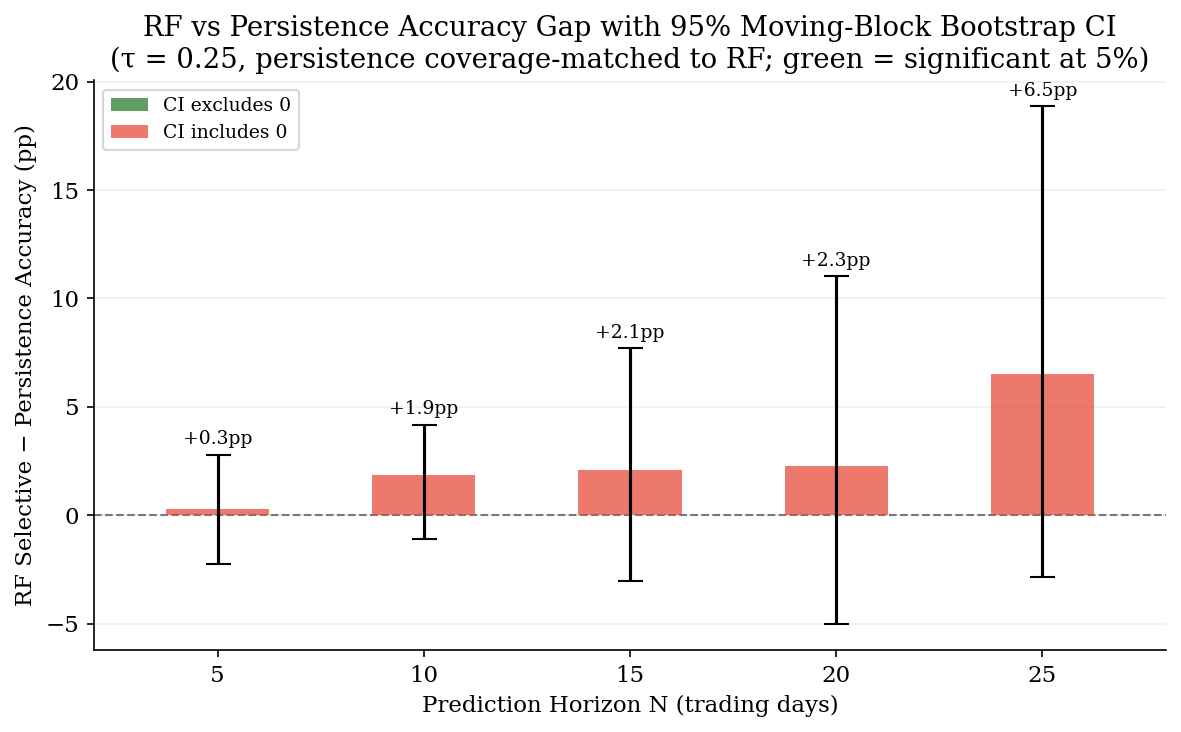
\includegraphics[width=0.75\textwidth]{bootstrap_ci.png}
\caption{Moving-block bootstrap 95\% confidence intervals for the RF-minus-persistence
selective accuracy gap across horizons. All intervals contain zero.}
\label{fig:bootstrap}
\end{figure}

The McNemar test at $N \geq 10$ finds $b = c = 0$: RF and persistence make
\emph{identical} predictions on every jointly covered day. This is a
deterministic result: once both systems decide to predict, they always agree.
The entire selective accuracy gap between RF and persistence is attributable
to differing abstention patterns, not differing predictions on shared days.

\subsection{Regime Transition Analysis}
\label{sec:transitions}

Table~\ref{tab:transitions} disaggregates RF performance by true regime
transition type at $N=5$. The calm$\to$calm and high$\to$high cells---the
persistence-stable transitions---achieve 99.6\% and 99.4\% accuracy
respectively at high coverage. The transition cells tell the opposite story.

\begin{table}[t]
\centering
\caption{RF coverage and accuracy by regime transition type ($N=5$, $\tau=0.25$).}
\label{tab:transitions}
\begin{tabular}{lrrrr}
\toprule
Transition & Total Days & Covered & Coverage & Acc (covered) \\
\midrule
calm $\to$ calm & 614 & 535 & 87.1\% & 99.6\% \\
calm $\to$ high & 79  & 36  & 45.6\% & \textbf{0.0\%}  \\
high $\to$ calm & 84  & 30  & 35.7\% & 23.3\% \\
high $\to$ high & 222 & 161 & 72.5\% & 99.4\% \\
\bottomrule
\end{tabular}
\end{table}

The confidence filter covers 36 of 79 calm$\to$high days---and issues a
confident ``stay calm'' prediction on all 36. This is not a failure of
calibration or class weighting; it is informational. Calm-to-high transitions
are predominantly triggered by exogenous macro shocks (geopolitical events,
policy surprises, systemic liquidity events) that leave no advance signature
in daily price features. Figure~\ref{fig:transition} shows the transition
analysis across all horizons.

\begin{figure}[t]
\centering
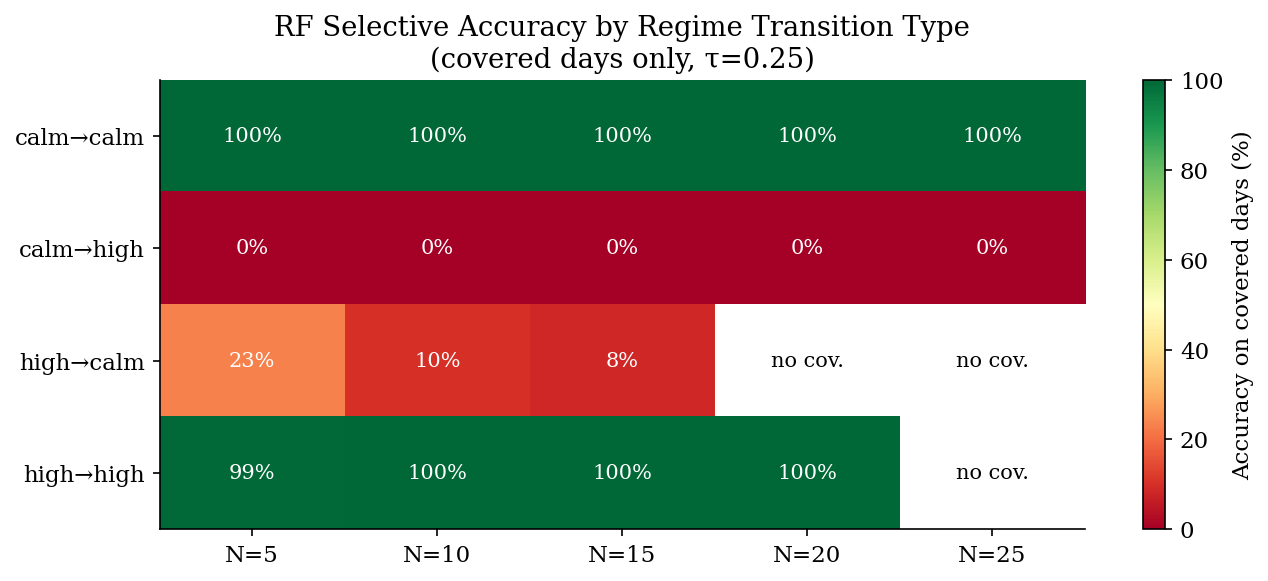
\includegraphics[width=\textwidth]{transition_analysis.png}
\caption{Coverage and accuracy by transition type across all prediction horizons.
Calm$\to$high covered accuracy is 0\% at every horizon.}
\label{fig:transition}
\end{figure}

\subsection{Cost-Weighted Utility and Abstention Analysis}

We define cost-weighted prediction utility as:
\begin{equation}
U(C) = -\frac{FP + C \cdot FN}{n_{\text{pred}}},
\end{equation}
where $C$ is the relative cost of a false negative (missed high-volatility
event). Under this measure, the RF selective framework is utility-beneficial
only when $C = 1$ (equal false positive and false negative costs) at $N=10$.
For $C \geq 5$---a conservative assumption for risk-averse applications---the
persistence baseline at matched coverage dominates RF at every horizon.
Explicit cost-weighting in the loss function up to $C = 20\times$ does not
rescue calm$\to$high covered accuracy: it remains 0.0\% at all weight levels
and all horizons, confirming the informational rather than objective-function
nature of the failure.

Figure~\ref{fig:abstention} illustrates the abstention confound: as the
threshold $\tau$ increases, coverage falls and the residual predictions
become progressively more persistence-dominated, with accuracy rising
mechanically.

\begin{figure}[t]
\centering
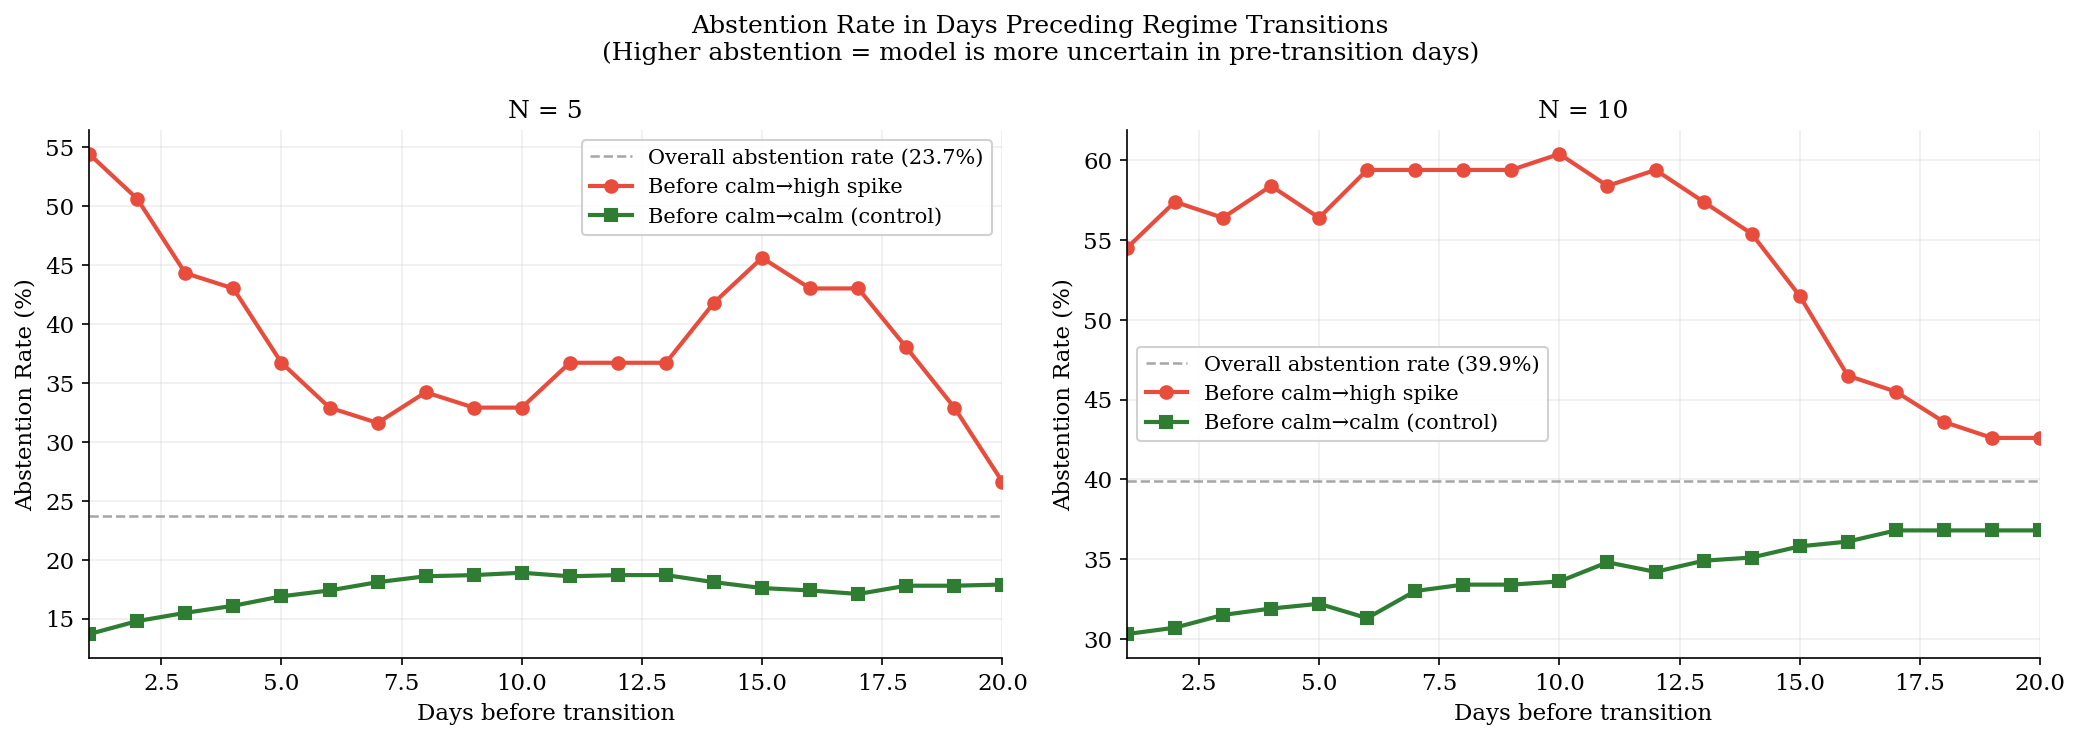
\includegraphics[width=0.75\textwidth]{abstention_analysis.png}
\caption{Coverage--accuracy tradeoff as abstention threshold $\tau$ increases.
Rising accuracy is driven by increasing persistence concentration, not improving
predictive skill.}
\label{fig:abstention}
\end{figure}

\subsection{SHAP Attribution and LSTM Comparison}
\label{sec:shap}

SHAP feature attribution~\cite{lundberg2017} at $N=5$ assigns 71.9\% of total
prediction mass to the 13 VIX technical features, with the dominant contributors
being the 20-day VIX mean (18.4\%), the 10-day VIX mean (14.2\%), and the
current VIX level (12.7\%). All three are smoothed or instantaneous
representations of VIX autocorrelation. Cross-asset features (gold, DXY,
Treasury yield slope) account for only 11.3\% of attribution mass despite
comprising 25\% of the feature set. At $N=10$, VIX technical attribution
falls to 64.7\%, with modest gains for macroeconomic features, but the
autocorrelation-dominant pattern persists. Figure~\ref{fig:shap} shows the
full SHAP importance decomposition.

\begin{figure}[t]
\centering
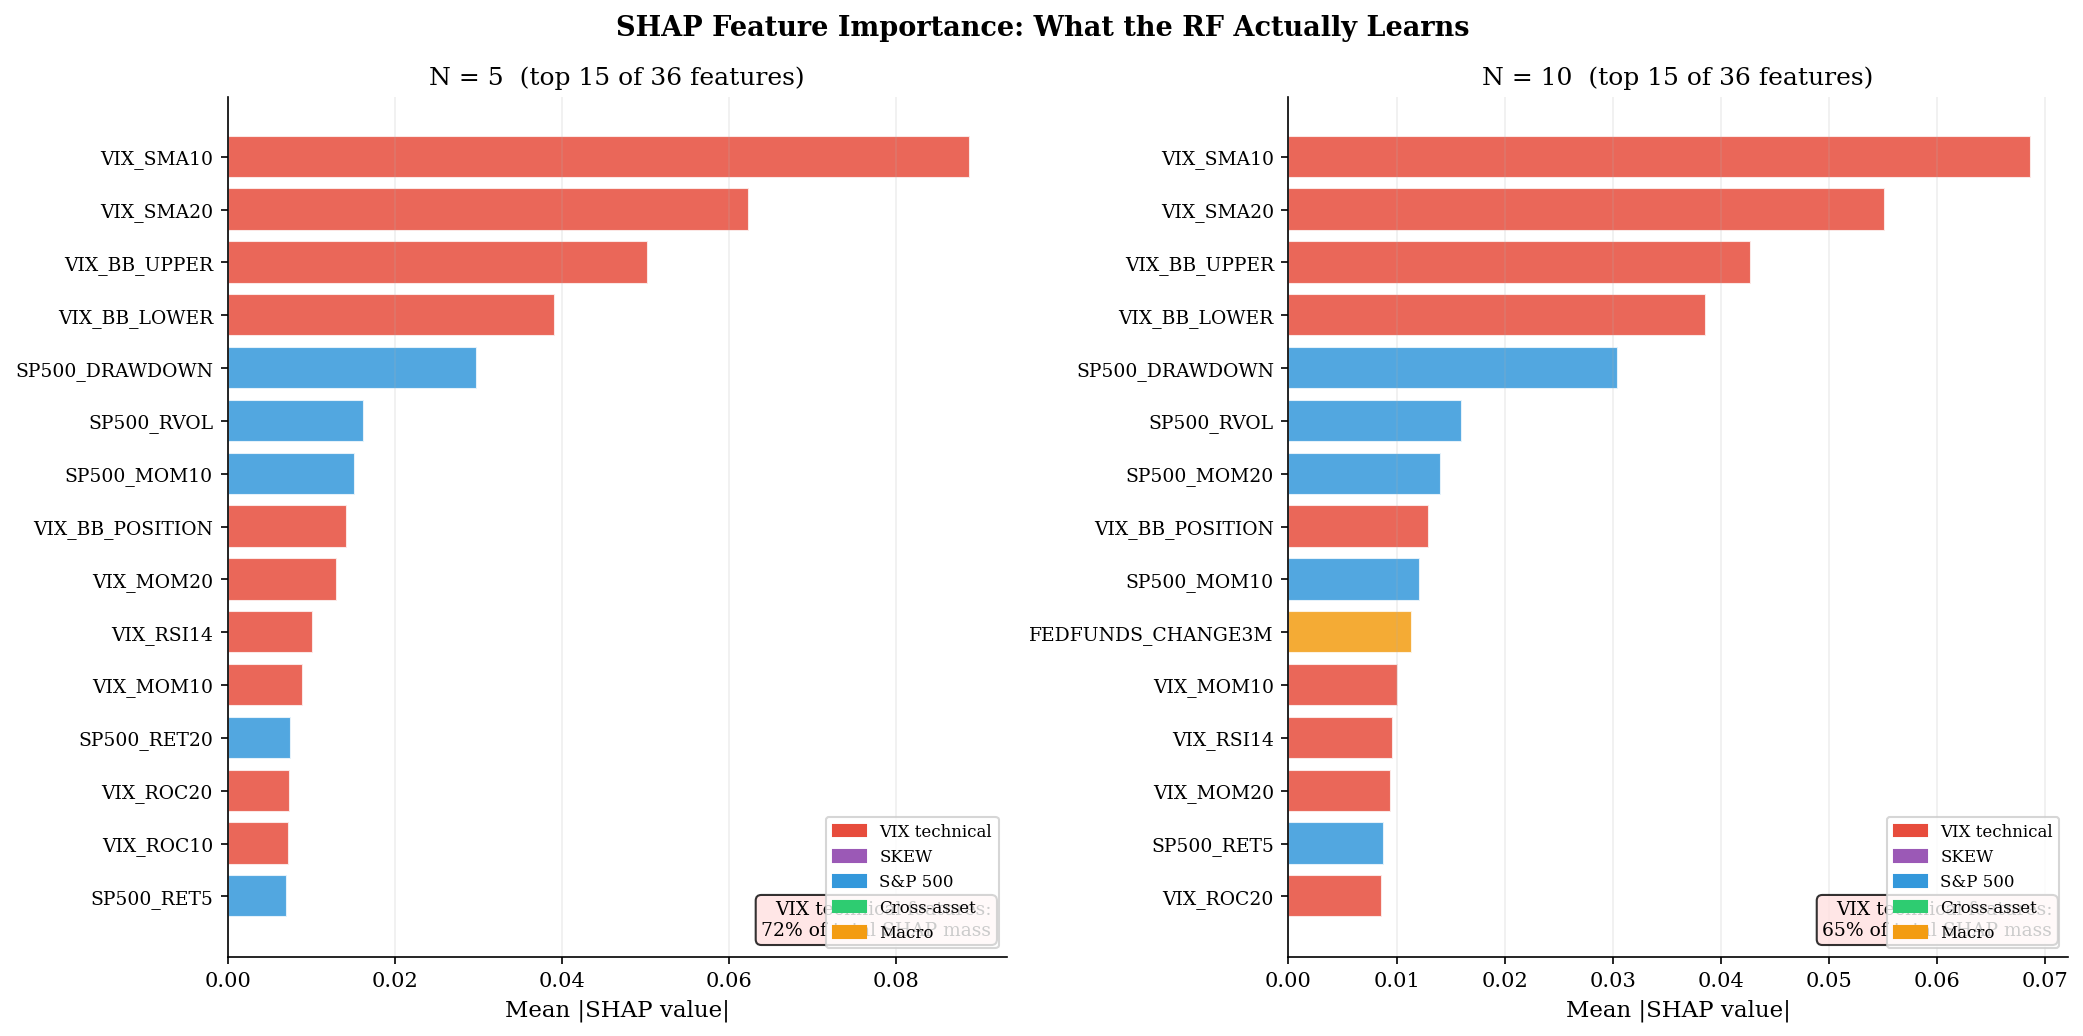
\includegraphics[width=0.75\textwidth]{shap_analysis.png}
\caption{SHAP feature importance at $N=5$. VIX technical features (autocorrelation
proxies) account for 71.9\% of total prediction mass.}
\label{fig:shap}
\end{figure}

A two-layer LSTM (hidden size 64, dropout 0.3, 20-day sliding window,
trained with focal loss to address class imbalance) achieves non-zero
calm$\to$high covered accuracy: 34.9\% at $N=5$. However, 34.9\% is
substantially below the 50\% random baseline, meaning the LSTM is wrong
more often than right on transition days. Temporal memory does not resolve
the informational constraint.

\subsection{S\&P 500 Replication}
\label{sec:sp500}

The full diagnostic replicates on S\&P~500 trend-regime classification,
where the binary label indicates whether the S\&P~500 index is above its
200-day moving average. The daily persistence ratio is $23.8\times$ at
$N=5$---more than twice the VIX ratio of $9.7\times$---reflecting the
lower intrinsic volatility of equity trend regimes. RF selective accuracy
reaches 86--92\% on S\&P~500 data but persistence dominates RF at every
horizon (RF minus persistence: $-4.0$ to $-7.1$~pp). Bull$\to$bear
covered accuracy is 0.0\% at $N=5$ and $N=10$, exactly replicating the
VIX calm$\to$high finding. Figure~\ref{fig:sp500} shows the replication
summary.

\begin{figure}[t]
\centering
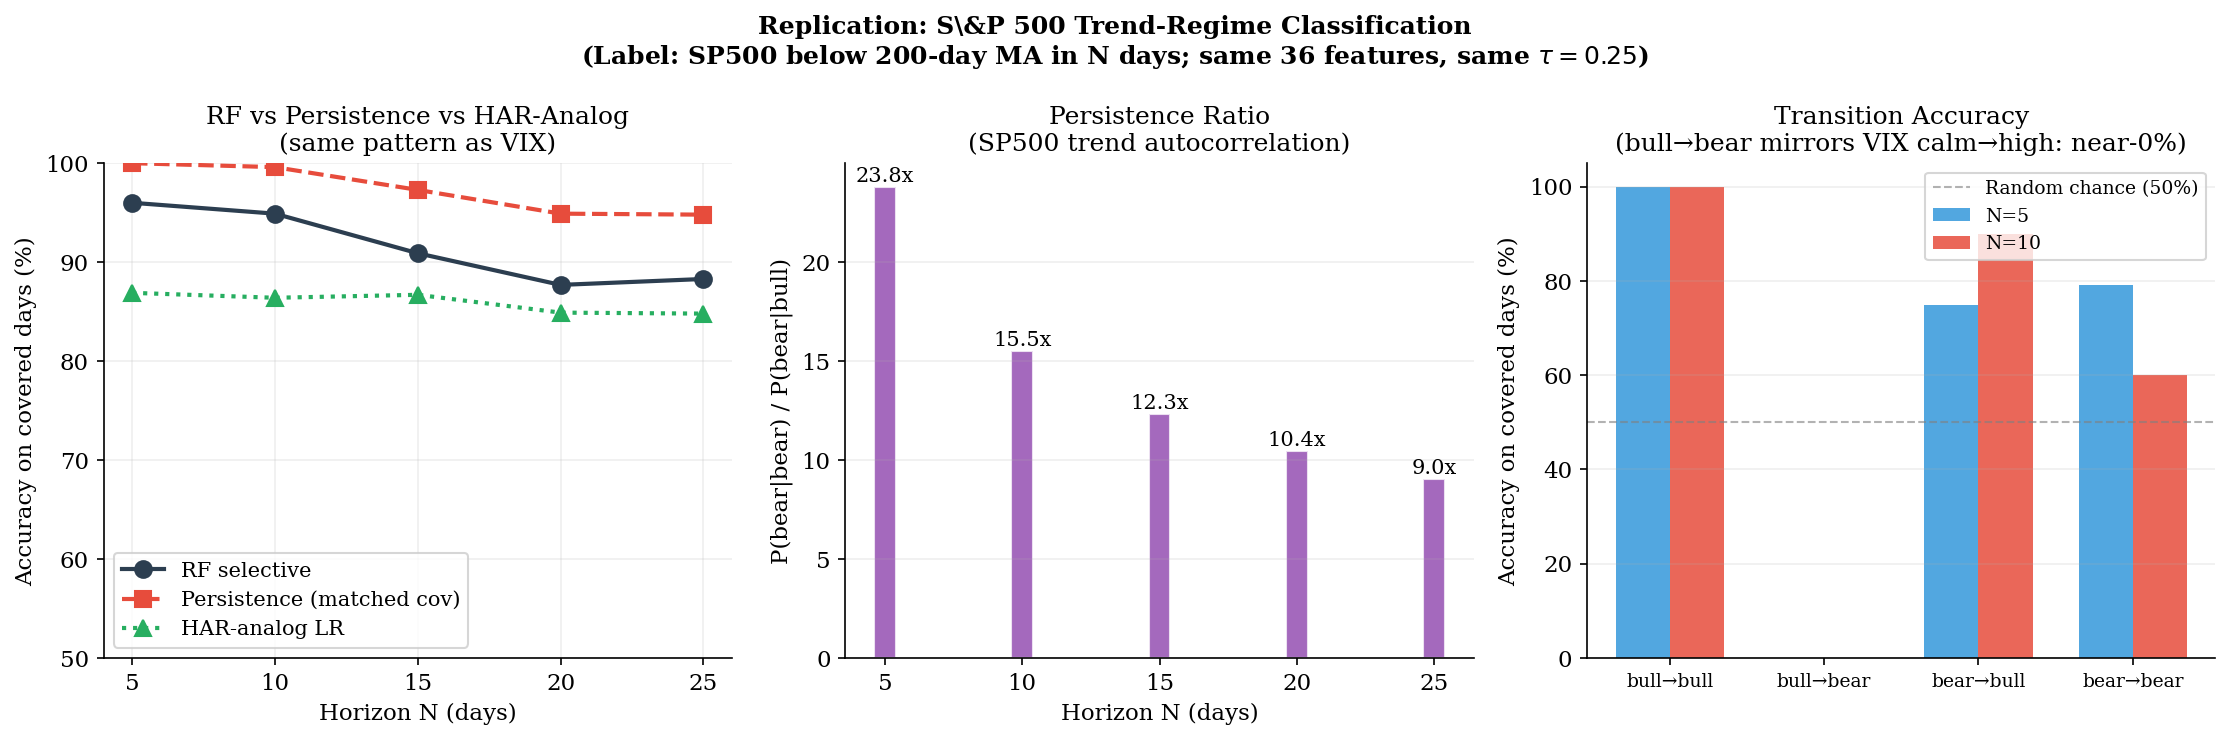
\includegraphics[width=0.75\textwidth]{sp500_replication.png}
\caption{S\&P~500 replication: selective accuracy vs.\ persistence baseline
and transition-type breakdown. The persistence illusion replicates structurally.}
\label{fig:sp500}
\end{figure}

The persistence illusion is therefore a structural consequence of applying
confidence-based selective prediction to any sufficiently autocorrelated
binary time series, not an artifact of VIX-specific data properties.


\section{Discussion}

\paragraph{Why the illusion persists.}
The mechanism is straightforward once identified. On financial regime data,
successive observations are highly correlated: daily VIX regime persistence
is approximately 97\% (transitions occur fewer than 3\% of trading days).
A classifier that learns this autocorrelation will assign high confidence to
regime-stable predictions and low confidence to transition predictions. The
selective prediction rule then preferentially covers stable days, where both
the classifier and persistence are correct. The resulting accuracy figure
reflects the persistence rate of the covered subset, not the classifier's
genuine discriminative ability.

\paragraph{The HAR diagnostic.}
The HAR-LR result carries a strong implication: if a three-feature model
using only current VIX, 5-day VIX mean, and 20-day VIX mean matches a
36-feature Random Forest, then the forest is not using its additional 33
features for genuine prediction---it is approximating the same HAR-style
autocorrelation with a more complex functional form. This is a qualitatively
different conclusion from ``the model is good'': it implies that feature
engineering, cross-asset data collection, and model complexity are unnecessary
for the observed accuracy level.

\paragraph{Practical implications for risk management.}
The 0\% calm$\to$high accuracy is the most consequential finding for
risk managers. Volatility regime transitions are precisely the events that
selective prediction systems should catch: unexpected spikes in VIX from
calm environments are the tail-risk scenarios that drive hedging demand
and portfolio drawdowns. A system that abstains on 54\% of those days and
issues a confident wrong prediction on the remaining 46\% is not only
unhelpful---it is actively misleading. Any real-world deployment must
evaluate calm$\to$high coverage and accuracy explicitly, not rely on
aggregate selective accuracy as a quality signal.

\paragraph{Generalizability of the diagnostic.}
The six-component protocol is designed to be transferable. Any selective
prediction system on autocorrelated binary time series should report:
(i)~balanced accuracy alongside selective accuracy; (ii)~baseline comparison
at matched coverage; (iii)~McNemar test on jointly covered days;
(iv)~transition-type accuracy disaggregation; (v)~SHAP or equivalent
attribution to detect autocorrelation exploitation; and
(vi)~cost-weighted utility under plausible false-negative cost ratios.
The absence of any of these six components leaves open the possibility that
reported accuracy reflects the persistence illusion.


\section{Limitations}

Our analysis is limited to VIX threshold classification at $\theta = 20$;
alternative thresholds (e.g., 15 or 25) would shift class prevalence and
persistence rates but are unlikely to alter the structural finding. The
feature set, while comprehensive, does not include options market microstructure
data, order flow, or high-frequency signals; it is possible that information
available at sub-daily frequency could improve transition detection. The
LSTM architecture tested is relatively shallow; more sophisticated sequence
models (Transformer-based, attention-augmented) might improve calm$\to$high
recall, though results suggest the bottleneck is informational rather than
architectural. The S\&P~500 replication uses only one alternative series;
further replication on other autocorrelated financial time series (credit
spreads, currency regimes) would strengthen the generalizability claim.


\section{Conclusion}

This paper applies a six-component diagnostic protocol to VIX regime
classification and demonstrates that headline selective prediction accuracy
of 90--93\% reflects autocorrelation, not machine learning skill.
A McNemar test finds $b = c = 0$ at $N \geq 10$, confirming that Random
Forest and persistence make identical predictions on every jointly covered
day. A three-feature HAR logistic regression matches or exceeds a 36-feature
Random Forest at four of five horizons under bootstrap testing. The confidence
filter achieves 0\% accuracy on calm$\to$high transitions at all horizons;
cost-weighting up to $20\times$ does not improve this. SHAP attributes 71.9\%
of prediction mass to VIX autocorrelation features; a two-layer LSTM also
fails on transition days. The full diagnostic replicates on S\&P~500 trend
regimes, establishing the persistence illusion as a structural property of
selective prediction on serially correlated binary labels.

The diagnostic protocol presented here is modular and directly applicable to
any selective prediction system on autocorrelated outcomes. Transparent
reporting of the six diagnostic components should be a prerequisite for
publishing or deploying selective prediction systems in financial risk
management contexts.

\paragraph{Acknowledgements.}
During the preparation of this work the authors used Claude (Anthropic) in
order to improve the readability and clarity of the manuscript. The authors
reviewed and edited the content as needed and take full responsibility for
the content of the publication.

\bibliographystyle{splncs04}
\bibliography{refs}

\end{document}
